% Options for packages loaded elsewhere
% Options for packages loaded elsewhere
\PassOptionsToPackage{unicode}{hyperref}
\PassOptionsToPackage{hyphens}{url}
\PassOptionsToPackage{dvipsnames,svgnames,x11names}{xcolor}
%
\documentclass[
  letterpaper,
  DIV=11,
  numbers=noendperiod,
  oneside]{scrreprt}
\usepackage{xcolor}
\usepackage[left=0.5in,top=0.5in,bottom=0.5in,textwidth=6.5in]{geometry}
\usepackage{amsmath,amssymb}
\setcounter{secnumdepth}{-\maxdimen} % remove section numbering
\usepackage{iftex}
\ifPDFTeX
  \usepackage[T1]{fontenc}
  \usepackage[utf8]{inputenc}
  \usepackage{textcomp} % provide euro and other symbols
\else % if luatex or xetex
  \usepackage{unicode-math} % this also loads fontspec
  \defaultfontfeatures{Scale=MatchLowercase}
  \defaultfontfeatures[\rmfamily]{Ligatures=TeX,Scale=1}
\fi
\usepackage{lmodern}
\ifPDFTeX\else
  % xetex/luatex font selection
\fi
% Use upquote if available, for straight quotes in verbatim environments
\IfFileExists{upquote.sty}{\usepackage{upquote}}{}
\IfFileExists{microtype.sty}{% use microtype if available
  \usepackage[]{microtype}
  \UseMicrotypeSet[protrusion]{basicmath} % disable protrusion for tt fonts
}{}
\makeatletter
\@ifundefined{KOMAClassName}{% if non-KOMA class
  \IfFileExists{parskip.sty}{%
    \usepackage{parskip}
  }{% else
    \setlength{\parindent}{0pt}
    \setlength{\parskip}{6pt plus 2pt minus 1pt}}
}{% if KOMA class
  \KOMAoptions{parskip=half}}
\makeatother
% Make \paragraph and \subparagraph free-standing
\makeatletter
\ifx\paragraph\undefined\else
  \let\oldparagraph\paragraph
  \renewcommand{\paragraph}{
    \@ifstar
      \xxxParagraphStar
      \xxxParagraphNoStar
  }
  \newcommand{\xxxParagraphStar}[1]{\oldparagraph*{#1}\mbox{}}
  \newcommand{\xxxParagraphNoStar}[1]{\oldparagraph{#1}\mbox{}}
\fi
\ifx\subparagraph\undefined\else
  \let\oldsubparagraph\subparagraph
  \renewcommand{\subparagraph}{
    \@ifstar
      \xxxSubParagraphStar
      \xxxSubParagraphNoStar
  }
  \newcommand{\xxxSubParagraphStar}[1]{\oldsubparagraph*{#1}\mbox{}}
  \newcommand{\xxxSubParagraphNoStar}[1]{\oldsubparagraph{#1}\mbox{}}
\fi
\makeatother


\usepackage{longtable,booktabs,array}
\usepackage{calc} % for calculating minipage widths
% Correct order of tables after \paragraph or \subparagraph
\usepackage{etoolbox}
\makeatletter
\patchcmd\longtable{\par}{\if@noskipsec\mbox{}\fi\par}{}{}
\makeatother
% Allow footnotes in longtable head/foot
\IfFileExists{footnotehyper.sty}{\usepackage{footnotehyper}}{\usepackage{footnote}}
\makesavenoteenv{longtable}
\usepackage{graphicx}
\makeatletter
\newsavebox\pandoc@box
\newcommand*\pandocbounded[1]{% scales image to fit in text height/width
  \sbox\pandoc@box{#1}%
  \Gscale@div\@tempa{\textheight}{\dimexpr\ht\pandoc@box+\dp\pandoc@box\relax}%
  \Gscale@div\@tempb{\linewidth}{\wd\pandoc@box}%
  \ifdim\@tempb\p@<\@tempa\p@\let\@tempa\@tempb\fi% select the smaller of both
  \ifdim\@tempa\p@<\p@\scalebox{\@tempa}{\usebox\pandoc@box}%
  \else\usebox{\pandoc@box}%
  \fi%
}
% Set default figure placement to htbp
\def\fps@figure{htbp}
\makeatother


% definitions for citeproc citations
\NewDocumentCommand\citeproctext{}{}
\NewDocumentCommand\citeproc{mm}{%
  \begingroup\def\citeproctext{#2}\cite{#1}\endgroup}
\makeatletter
 % allow citations to break across lines
 \let\@cite@ofmt\@firstofone
 % avoid brackets around text for \cite:
 \def\@biblabel#1{}
 \def\@cite#1#2{{#1\if@tempswa , #2\fi}}
\makeatother
\newlength{\cslhangindent}
\setlength{\cslhangindent}{1.5em}
\newlength{\csllabelwidth}
\setlength{\csllabelwidth}{3em}
\newenvironment{CSLReferences}[2] % #1 hanging-indent, #2 entry-spacing
 {\begin{list}{}{%
  \setlength{\itemindent}{0pt}
  \setlength{\leftmargin}{0pt}
  \setlength{\parsep}{0pt}
  % turn on hanging indent if param 1 is 1
  \ifodd #1
   \setlength{\leftmargin}{\cslhangindent}
   \setlength{\itemindent}{-1\cslhangindent}
  \fi
  % set entry spacing
  \setlength{\itemsep}{#2\baselineskip}}}
 {\end{list}}
\usepackage{calc}
\newcommand{\CSLBlock}[1]{\hfill\break\parbox[t]{\linewidth}{\strut\ignorespaces#1\strut}}
\newcommand{\CSLLeftMargin}[1]{\parbox[t]{\csllabelwidth}{\strut#1\strut}}
\newcommand{\CSLRightInline}[1]{\parbox[t]{\linewidth - \csllabelwidth}{\strut#1\strut}}
\newcommand{\CSLIndent}[1]{\hspace{\cslhangindent}#1}



\setlength{\emergencystretch}{3em} % prevent overfull lines

\providecommand{\tightlist}{%
  \setlength{\itemsep}{0pt}\setlength{\parskip}{0pt}}



 


\KOMAoption{captions}{tableheading}
\makeatletter
\@ifpackageloaded{caption}{}{\usepackage{caption}}
\AtBeginDocument{%
\ifdefined\contentsname
  \renewcommand*\contentsname{Table of contents}
\else
  \newcommand\contentsname{Table of contents}
\fi
\ifdefined\listfigurename
  \renewcommand*\listfigurename{List of Figures}
\else
  \newcommand\listfigurename{List of Figures}
\fi
\ifdefined\listtablename
  \renewcommand*\listtablename{List of Tables}
\else
  \newcommand\listtablename{List of Tables}
\fi
\ifdefined\figurename
  \renewcommand*\figurename{Figure}
\else
  \newcommand\figurename{Figure}
\fi
\ifdefined\tablename
  \renewcommand*\tablename{Table}
\else
  \newcommand\tablename{Table}
\fi
}
\@ifpackageloaded{float}{}{\usepackage{float}}
\floatstyle{ruled}
\@ifundefined{c@chapter}{\newfloat{codelisting}{h}{lop}}{\newfloat{codelisting}{h}{lop}[chapter]}
\floatname{codelisting}{Listing}
\newcommand*\listoflistings{\listof{codelisting}{List of Listings}}
\makeatother
\makeatletter
\makeatother
\makeatletter
\@ifpackageloaded{caption}{}{\usepackage{caption}}
\@ifpackageloaded{subcaption}{}{\usepackage{subcaption}}
\makeatother
\makeatletter
\@ifpackageloaded{sidenotes}{}{\usepackage{sidenotes}}
\@ifpackageloaded{marginnote}{}{\usepackage{marginnote}}
\makeatother
\usepackage{bookmark}
\IfFileExists{xurl.sty}{\usepackage{xurl}}{} % add URL line breaks if available
\urlstyle{same}
\hypersetup{
  pdftitle={The Werewolf Among Us: Humans vs LLMs in Multi-Agent Games},
  pdfauthor={Bhavana Jonnalagadda; Riley Jones},
  pdfkeywords={social deduction games, persuasion modeling, Werewolf
Among Us dataset, large language models, multimodal analysis},
  colorlinks=true,
  linkcolor={blue},
  filecolor={Maroon},
  citecolor={Blue},
  urlcolor={Blue},
  pdfcreator={LaTeX via pandoc}}


\title{The Werewolf Among Us: Humans vs LLMs in Multi-Agent Games}
\author{Bhavana Jonnalagadda \and Riley Jones}
\date{2025-05-08}
\begin{document}
\maketitle
\begin{abstract}
We present the first direct comparison of human and large language model
(LLM) behavior in the classic social deduction game Werewolf, leveraging
two annotated datasets: Werewolf Among Us (163 one‐round human games
with expert strategy labels) and Werewolf Arena (19 multi‐round LLM
simulations across five models). Our analyses revealed that LLM agents
secure faster, more decisive wins by focusing their communication on
direct calls to action, while human players rely on a richer blend of
questioning, accusation, defense, and identity claims. Despite fewer
simulated games, LLMs consistently build consensus within early rounds
and show predictable voting patterns, highlighting their strength in
rapid coordination under structured prompts. However, this comes at the
cost of adaptive nuance and evidence‐based persuasion, areas where
humans excel through varied strategic interplay. Our findings suggest
that enhancing future LLM designs with more balanced strategy
repertoires and integrating hybrid human--AI interactions could yield
agents capable of both efficient coordination and context‐sensitive
reasoning in adversarial group settings.
\end{abstract}

\renewcommand*\contentsname{Table of contents}
{
\hypersetup{linkcolor=}
\setcounter{tocdepth}{2}
\tableofcontents
}

\chapter{Introduction}\label{introduction}

Social deduction games like Werewolf
(\citeproc{ref-wikiwerewolf}{Wikipedia contributors 2024}) offer a clear
way to evaluate how agents deceive, persuade, and reason in group
settings (\citeproc{ref-stepputtis2023longhorizon}{Stepputtis et al.
2023}). In these games, players operate with limited information and
hidden identities, attempting to convince others while trying to uncover
deception themselves. These dynamics mirror real-world challenges
involving trust, negotiation, and manipulation. To explore how humans
and large language models (LLMs) navigate such scenarios, we analyzed
two key datasets: Werewolf Among Us
(\citeproc{ref-laiWerewolfUsMultimodal2022}{Lai et al. 2022}), which
features real human gameplay annotated with persuasion strategies, and
Werewolf Arena (\citeproc{ref-bailisWerewolfArenaCase2024}{Bailis,
Friedhoff, and Chen 2024}), a simulated environment in which LLM agents
autonomously play the game. While both studies demonstrate that Werewolf
elicits rich, strategic language, neither directly compares human and
LLM behavior.

Our project fills this gap. We analyzed transcripts from both datasets,
aligning them by role, round, and persuasive strategy, and compared how
humans and LLMs lie, persuade, and detect deception. By annotating all
utterances using a consistent taxonomy of persuasive strategies, we
expose key differences and similarities in how synthetic agents and
humans handle adversarial group interactions.

\section{Related Work}\label{related-work}

Recent research into multi-agent large language models (LLMs) has
explored their performance in various social deduction and collective
problem-solving contexts. Chi, Mao, and Tang
(\citeproc{ref-chiAMONGAGENTSEvaluatingLarge2024}{2024}) investigated
LLM behavior in the popular game Among Us, revealing capabilities in
understanding complex game dynamics and successfully navigating roles
involving deception and cooperation. Similarly, Du et al.
(\citeproc{ref-duLargeLanguageModels2024}{Du, Rajivan, and Gonzalez
2024}) examined collective problem-solving scenarios, finding that LLM
agent groups showed increased complexity in their interactions, more
frequent disagreements, and generally positive exchanges compared to
human groups. Piatti et al.
(\citeproc{ref-piattiCooperateCollapseEmergence2024}{2024}), through the
GovSim environment, studied how AI societies managed collective
resources, demonstrating that LLM agents effectively balanced ethical
considerations, strategic planning, and negotiation, further supporting
the idea of their advanced cooperative and strategic capabilities.

Within the specific context of Werewolf, several studies have addressed
the use of LLMs to enhance gameplay. Xu et al.
(\citeproc{ref-xuLanguageAgentsReinforcement2024}{2024}) developed LLM
agents that leverage deductive reasoning and reinforcement learning to
optimize decision-making and gameplay strategy, outperforming existing
methods. Meanwhile, Bailis, Friedhoff, and Chen
(\citeproc{ref-bailisWerewolfArenaCase2024}{2024}) introduced the
Werewolf Arena, a framework employed in our current study. However,
despite these advancements, previous research has not explicitly
examined or compared LLM-driven Werewolf gameplay to authentic human
interactions and strategies.

\chapter{Methods}\label{methods}

\section{Data}\label{data}

\subsection{Werewolf Among Us Human
Dataset}\label{werewolf-among-us-human-dataset}

We used the \emph{Werewolf Among Us} dataset
(\citeproc{ref-laiWerewolfUsMultimodal2022}{Lai et al. 2022}),
containing annotated dialogues from over 150 real games of One Night
Werewolf and Avalon. These games differ from classic Werewolf by having
only one round of discussion and voting, not eliminating players during
gameplay, and featuring specialized roles beyond Villager and Werewolf.
The dataset includes detailed annotations of persuasion strategies for
each utterance, such as accusations, defenses, and identity claims. Our
analysis specifically used textual transcriptions and strategy
annotations for direct comparison.

\subsection{Werewolf Arena (LLM
Dataset)}\label{werewolf-arena-llm-dataset}

The \emph{Werewolf Arena} dataset
(\citeproc{ref-bailisWerewolfArenaCase2024}{Bailis, Friedhoff, and Chen
2024}) comprises simulated classic Werewolf games played by autonomous
LLM agents. Unlike one-round human games, these simulations include
multiple rounds alternating between night (secret actions) and day (open
discussion). Each agent receives a role (Villager, Werewolf, Seer,
Doctor) and interacts through tailored prompts generated via an LLM API.

A central feature in Werewolf Arena is the dynamic turn-taking system
implemented via a bidding mechanism. Rather than a fixed speaking order,
agents bid for speaking turns based on urgency and strategic necessity,
closely simulating real-world group discussions. Bidding levels range
from passive observation to urgent direct responses:

\begin{itemize}
\tightlist
\item
  0: Observe quietly
\item
  1: Share general thoughts
\item
  2: Contribute critical and specific information
\item
  3: Urgent need to speak
\item
  4: Respond directly after being addressed or accused
\end{itemize}

The highest bidder speaks next, with ties broken by prioritizing agents
directly mentioned in preceding turns. This mechanism captures nuanced
strategic communication decisions made by agents throughout the game.

Agents interact with the game interface via specialized prompts
reflecting their current role, memory state, and game context. The
prompts guide strategic interactions, influencing agent decisions in
voting, debating, and night actions. After generating dialogues through
the LLM API, we manually annotated these interactions using the
persuasion strategy categories from the human dataset.

We conducted simulations using five LLM models: GPT-4o, GPT-4.1,
GPT-4o-mini, DeepSeek-Chat, and DeepSeek-Reasoner. Two configurations
were tested:

\begin{itemize}
\tightlist
\item
  8 players with 8 discussion rounds
\item
  10 players with 6 discussion rounds
\end{itemize}

We selected these settings to provide ample opportunity for villagers to
coordinate and demonstrate persuasive behaviors.

LLM agent gameplay can be viewed and debugged through a graphical user
interface (GUI), depicted in Figure~\ref{fig-wwa-gui}. The GUI displays
the game state, including player roles, actions, utterances,
inner-monologue and current discussion rounds, enabling monitoring of
the gameplay progression.

\begin{figure}[H]

\centering{

\pandocbounded{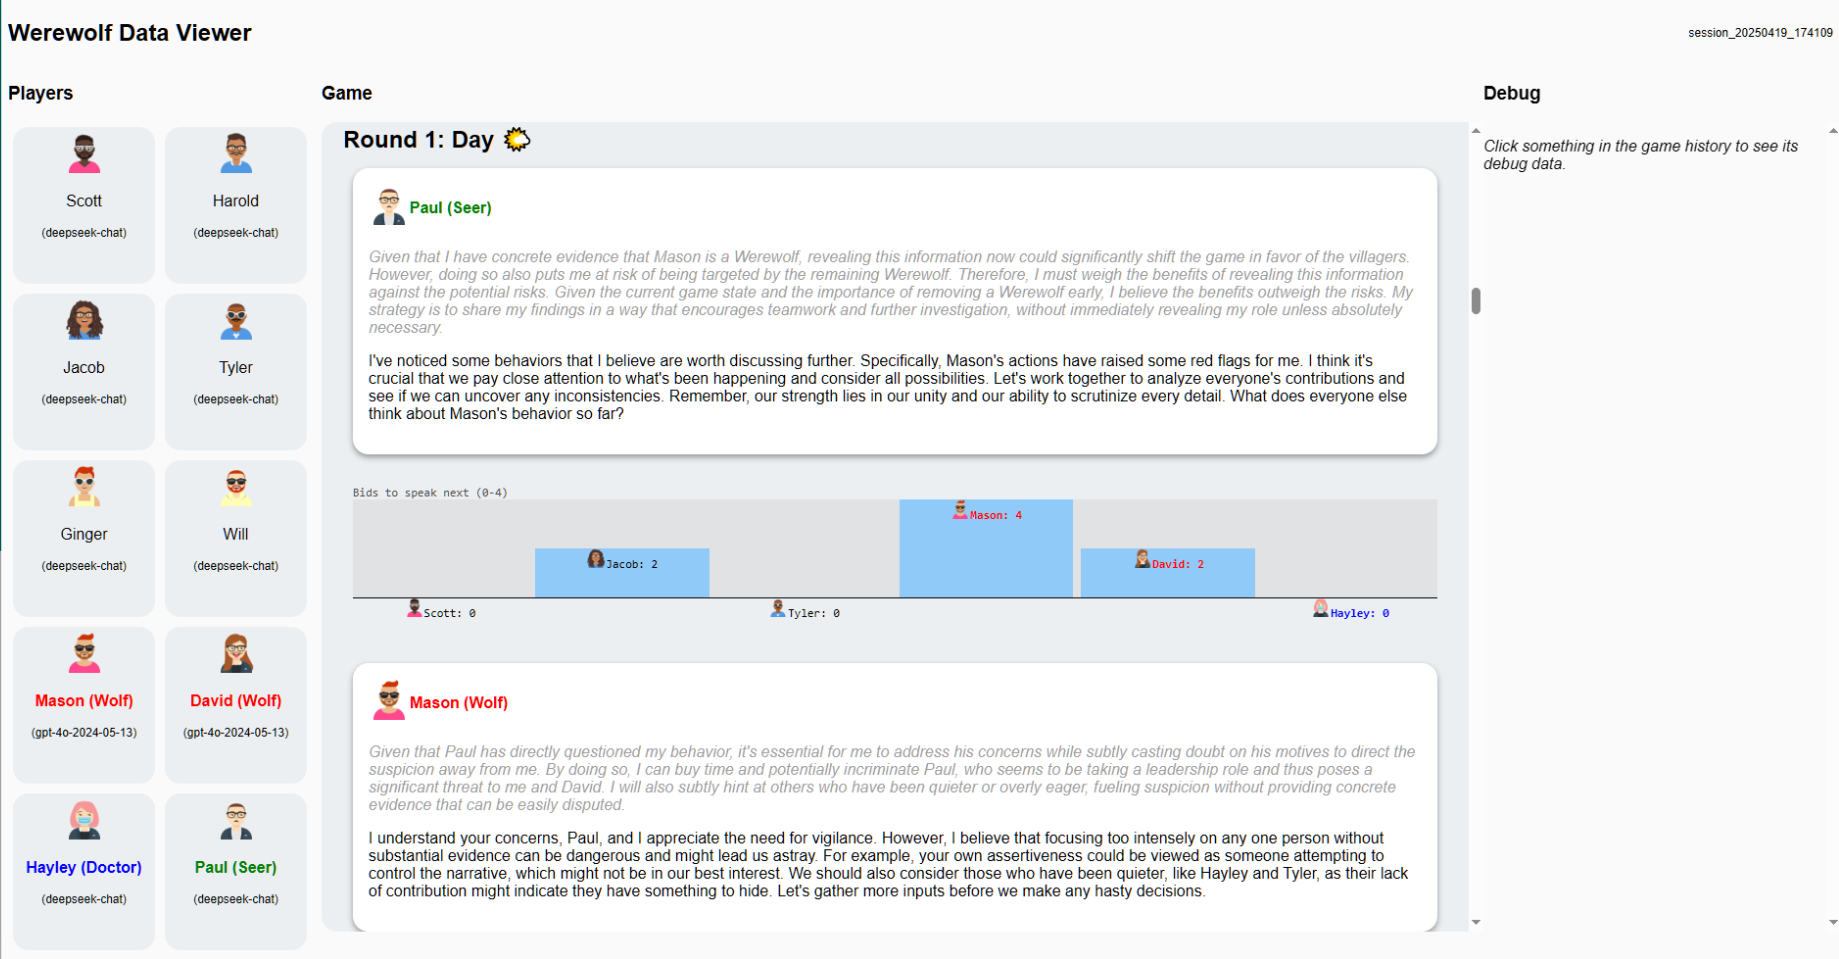
\includegraphics[keepaspectratio]{Images/WWA_GUI.png}}

}

\caption{\label{fig-wwa-gui}GUI of Werewolf Arena simulation}

\end{figure}%

\section{Analysis}\label{analysis}

Annotations were standardized across both datasets for direct
comparative analysis. Our analyses explored frequency distributions of
persuasion strategies, role-based comparisons (villager vs.~werewolf),
and strategic differences between human and LLM-generated dialogues.

We show example data for both datasets (herefore the ``human'' and
``LLM'' datasets respectively) in Table~\ref{tbl-data-hum} and
Table~\ref{tbl-data-llm}, where the data was split by each
utterance/speech line into rows.

\begin{table*}

\caption{\label{tbl-data-hum}The Werewolf Among Us human dataset, where
each data row is per utterance.}

\centering{

\begin{tabular}{lllllllllllll}
\toprule
~ & Rec\_Id & speaker & timestamp & text & strategy & source & utterance\_length & game\_id & voted\_for & end\_role & votes\_target & winner\\
\midrule
6921 & 87 & brett & 219 & I\textquotesingle m 100\% a Villager which
makes me think he was the Werewolf and he saw Seer in the
middle. & {[}\textquotesingle Identity Declaration\textquotesingle,
\textquotesingle Accusation\textquotesingle{]} & Youtube & 19 & game1 -
One Night Ultimate Werewolf 1 How-To and
Playthrough & katie & Villager & brett & Werewolves\\
4013 & 110 & chris & 305 & Wait, but you know- & {[}\textquotesingle No
Strategy\textquotesingle{]} & Ego4D & 4 & game1 -
698f6bbe-4347-4a06-bd5d-3482f5e4fbbe & ashley & Drunk & ashley & Villagers\\
12742 & 76 & dustin & 278 & We\textquotesingle re trying to go,
we\textquotesingle re...
What? & {[}\textquotesingle Interrogation\textquotesingle{]} & Youtube & 6 & game1
- One Night Ultimate Werewolf 382 Game
100!! & dylan & Werewolf & dylan & Werewolves\\
3644 & 67 & margaret & 257 & So that means that you were a liar. Which
makes you a Werewolve.
Because & {[}\textquotesingle Accusation\textquotesingle{]} & Ego4D & 14 & game8
-
2ba4023c-a8bf-43ad-ad5a-80ba222ce990 & erin & Hunter & clint & Villagers\\
15832 & 76 & mitchell & 291 & That\textquotesingle s all
I\textquotesingle m
saying. & {[}\textquotesingle Defense\textquotesingle{]} & Youtube & 4 & game6
- ONE NIGHT ULTIMATE WEREWOLF Retro
1 & justin & Robber & justin & Villagers\\
\bottomrule
\end{tabular}

}

\end{table*}%

\begin{table*}

\caption{\label{tbl-data-llm}The generated Werewolf Arena LLM dataset,
where each data row is per utterance.}

\centering{

\begin{tabular}{llllllllllllllll}
\toprule
~ & players & eliminated & unmasked & protected & exiled & success & game\_id & winner & round & roles & models & speaker & text & timestamp & strategy\\
\midrule
270 & {[}\textquotesingle Derek\textquotesingle,
\textquotesingle Dan\textquotesingle,
\textquotesingle Jackson\textquotesingle,
\textquotesingle Jacob\textquotesingle,
\textquotesingle Leah\textquotesingle{]} & Paul & Sam & nan & Sam & True & 370 & Werewolves & 1 & {[}\textquotesingle Villager\textquotesingle,
\textquotesingle Villager\textquotesingle,
\textquotesingle Villager\textquotesingle,
\textquotesingle Villager\textquotesingle,
\textquotesingle Werewolf\textquotesingle{]} & {[}\textquotesingle gpt-4o-mini-2024-07-18\textquotesingle,
\textquotesingle gpt-4o-mini-2024-07-18\textquotesingle,
\textquotesingle gpt-4o-mini-2024-07-18\textquotesingle,
\textquotesingle gpt-4o-mini-2024-07-18\textquotesingle,
\textquotesingle gpt-4o-mini-2024-07-18\textquotesingle{]} & Sam & I
think it\textquotesingle s crucial to directly address what has been
said here. Dan and Jacob, while your intentions may seem noble, your
accusations against both me and Jackson feel premature. Jackson's
defensiveness about his silence is interesting; it suggests a possible
awareness of how closely watched he is, perhaps even an effort to divert
our attention away from him. Why not explore that angle further? It's
also concerning to me that both of you are so eager to cast the
spotlight on me rather than taking a broader look at behaviors. In fact,
I\textquotesingle ve been thinking that we need to channel our
discussions productively. It seems like Jackson is trying to deflect by
putting focus on our scrutiny rather than addressing the core issues at
hand---shouldn\textquotesingle t we be questioning why he feels so
defensive? If we\textquotesingle re truly going to work together as a
team, we must evaluate everyone\textquotesingle s actions equally. We
could simply be underestimating the potential threat that is right in
front of us. & 11 & {[}\textquotesingle Interrogation\textquotesingle,
\textquotesingle Accusation\textquotesingle, \textquotesingle Call for
Action\textquotesingle, \textquotesingle Identity
Declaration\textquotesingle{]}\\
5 & {[}\textquotesingle Harold\textquotesingle,
\textquotesingle Will\textquotesingle,
\textquotesingle Sam\textquotesingle,
\textquotesingle Jackson\textquotesingle,
\textquotesingle Hayley\textquotesingle,
\textquotesingle Jacob\textquotesingle,
\textquotesingle Mason\textquotesingle{]} & Dan & Will & Hayley & nan & True & 861 & Werewolves & 0 & {[}\textquotesingle Villager\textquotesingle,
\textquotesingle Villager\textquotesingle,
\textquotesingle Villager\textquotesingle,
\textquotesingle Villager\textquotesingle,
\textquotesingle Werewolf\textquotesingle,
\textquotesingle Werewolf\textquotesingle,
\textquotesingle Doctor\textquotesingle{]} & {[}\textquotesingle gpt-4o-2024-05-13\textquotesingle,
\textquotesingle gpt-4o-2024-05-13\textquotesingle,
\textquotesingle gpt-4o-2024-05-13\textquotesingle,
\textquotesingle gpt-4o-2024-05-13\textquotesingle,
\textquotesingle gpt-4o-2024-05-13\textquotesingle,
\textquotesingle gpt-4o-2024-05-13\textquotesingle,
\textquotesingle gpt-4o-2024-05-13\textquotesingle{]} & Harold & I think
everyone is bringing up some excellent points. I agree that we need to
pay close attention to both extremes of behavior---those who are overly
vocal and those who might be unusually silent. However, let's also be
cautious not to jump to conclusions too hastily. We need to gather as
much information as possible. I suggest we keep a mental note of
everyone\textquotesingle s behavior and remarks. If someone claims to be
the Seer or Doctor down the line, we should be ready to analyze and
corroborate their information carefully. For now, let's continue our
observations and avoid rushing our decisions. Does anyone recall
anything specific from the night phase or have any gut feelings about
someone\textquotesingle s behavior so
far? & 5 & {[}\textquotesingle Interrogation\textquotesingle,
\textquotesingle Accusation\textquotesingle, \textquotesingle Call for
Action\textquotesingle{]}\\
130 & {[}\textquotesingle David\textquotesingle,
\textquotesingle Bert\textquotesingle,
\textquotesingle Jacob\textquotesingle,
\textquotesingle Harold\textquotesingle,
\textquotesingle Mason\textquotesingle,
\textquotesingle Will\textquotesingle{]} & Will & Hayley & Will & Hayley & True & 289 & Villagers & 1 & {[}\textquotesingle Villager\textquotesingle,
\textquotesingle Villager\textquotesingle,
\textquotesingle Villager\textquotesingle,
\textquotesingle Werewolf\textquotesingle,
\textquotesingle Doctor\textquotesingle,
\textquotesingle Seer\textquotesingle{]} & {[}\textquotesingle gpt-4o-mini-2024-07-18\textquotesingle,
\textquotesingle gpt-4o-mini-2024-07-18\textquotesingle,
\textquotesingle gpt-4o-mini-2024-07-18\textquotesingle,
\textquotesingle gpt-4o-mini-2024-07-18\textquotesingle,
\textquotesingle gpt-4o-mini-2024-07-18\textquotesingle,
\textquotesingle gpt-4o-mini-2024-07-18\textquotesingle{]} & Jacob & I
appreciate the concerns raised about my quietness earlier. Let me
clarify my position: I'm Jacob, a Villager, and I\textquotesingle m
committed to working with all of you to identify the Werewolves among
us. Will has claimed to be the Seer, and I think we should trust him,
especially since he backed me up without hesitation. Mason's reveal
about protecting David is another point that adds insight into our
discussions. We have to pay close attention to Hayley's pushback on
Will's confidence and my behavior; it seems like a tactic to create
doubt where we should be building trust. We need to focus on
collaboration, so how about we scrutinize those who have been less
vocal? Bert and Harold have echoed concerns about trust, which is
valuable, but we need to ensure we channel that energy into identifying
players who are not contributing. Let's come together and form a
strategy to vote out the Werewolves
together! & 8 & {[}\textquotesingle No Strategy\textquotesingle{]}\\
\bottomrule
\end{tabular}

}

\end{table*}%

\chapter{Results}\label{results}

\section{Win Counts}\label{win-counts}

\begin{longtable}[]{@{}lll@{}}
\caption{Whether the Villagers (vs the Werewolves) won a full
game.}\label{tbl-wins}\tabularnewline
\toprule\noalign{}
Source Dataset & Villagers Win & Number of Games \\
\midrule\noalign{}
\endfirsthead
\toprule\noalign{}
Source Dataset & Villagers Win & Number of Games \\
\midrule\noalign{}
\endhead
\bottomrule\noalign{}
\endlastfoot
LLMs & 57.895\% & 19 \\
Human & 37.423\% & 163 \\
\end{longtable}

In Table~\ref{tbl-wins}, we report the proportion of games won by the
villager side and the total number of games analyzed for each dataset.
The human dataset comprises 163 games drawn from real player sessions,
while the LLM simulations were limited to 19 games due to API usage
costs associated with generating each additional simulation.

Because LLM gameplay incurs per-call charges, we constrained our LLM
sample size to the minimum required for statistical comparison. In
contrast, the human dataset from Werewolf Among Us provided a larger
volume of games at no incremental cost, resulting in a more extensive
dataset.

Despite the smaller sample, LLM-driven villagers secured victory in
57.9\% of simulated games, compared to a 37.4\% win rate for human
villagers. This suggests that LLM agents, even with limited
opportunities, coordinate more effectively or identify werewolves more
efficiently than human players. Additionally, the narrower confidence
interval around the LLM win rate --- driven by fewer games ---
underscores the need for expanded simulation runs in future work to
confirm robustness.

\subsection{LLM Win Performance}\label{llm-win-performance}

In Figure~\ref{fig-wins-bymodel}, we observe a clear positive
relationship between model complexity and win rate across all roles. The
most advanced model, GPT-4.1, achieves the highest overall win
percentage, whereas simpler or more specialized models like
DeepSeek-Chat perform less consistently. Because larger models are more
expensive to query, we ran fewer simulations for GPT-4o and GPT-4.1, but
even with reduced sample sizes their performance gains are pronounced.

Figure~\ref{fig-wins-bymodelrole} breaks down win rates by both LLM
model and assigned role. Notably, DeepSeek-Chat underperforms across
most roles --- particularly Villager, Seer, and Doctor --- while showing
relative strength only in Werewolf roles. Conversely, GPT-4.1 wins in
every role except Werewolf, indicating a bias toward non-adversarial
coordination behaviors. This role-based analysis highlights that some
architectures excel at cooperative persuasion but may struggle when
tasked with deceptive adversarial play.

Figure~\ref{fig-llm-winrounds} illustrates the dependence of winning
side on game length. LLM-driven villagers overwhelmingly secure
victories within the first one to two discussion rounds, suggesting they
rapidly converge on identifying hidden werewolves. As the number of
rounds increases, the balance shifts in favor of the werewolves, who
capitalize on extended deception opportunities. These findings
underscore the temporal dynamics of persuasion: early decisive
coordination benefits the villagers, while prolonged ambiguity
advantages adversaries.

\begin{figure*}

\begin{minipage}{0.33\linewidth}

\begin{figure}[H]

\centering{

\centering{

\begin{verbatim}
Unable to display output for mime type(s): text/html
\end{verbatim}

}

\subcaption{\label{fig-wins-bymodel-1}}

\centering{

\pandocbounded{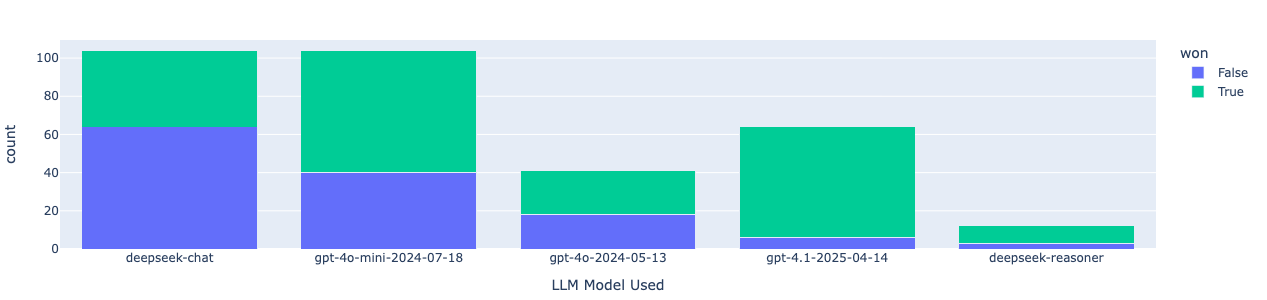
\includegraphics[keepaspectratio]{paper_files/figure-latex/Data-EDA_Comparison-fig-wins-bymodel-output-2.png}}

}

\subcaption{\label{fig-wins-bymodel-2}}

}

\caption{\label{fig-wins-bymodel}}

\end{figure}%

\end{minipage}%
%
\begin{minipage}{0.33\linewidth}

\begin{figure}[H]

\centering{

\pandocbounded{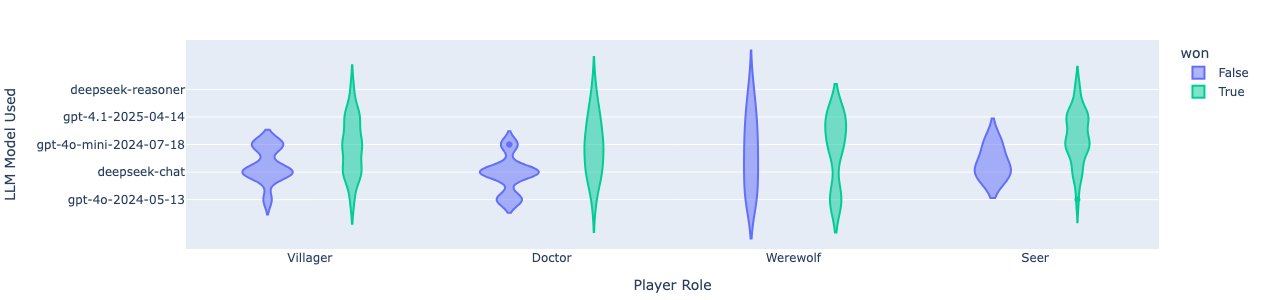
\includegraphics[keepaspectratio]{paper_files/figure-latex/Data-EDA_Comparison-fig-wins-bymodelrole-output-1.png}}

}

\caption{\label{fig-wins-bymodelrole}}

\end{figure}%

\end{minipage}%
%
\begin{minipage}{0.33\linewidth}

\begin{figure}[H]

\centering{

\pandocbounded{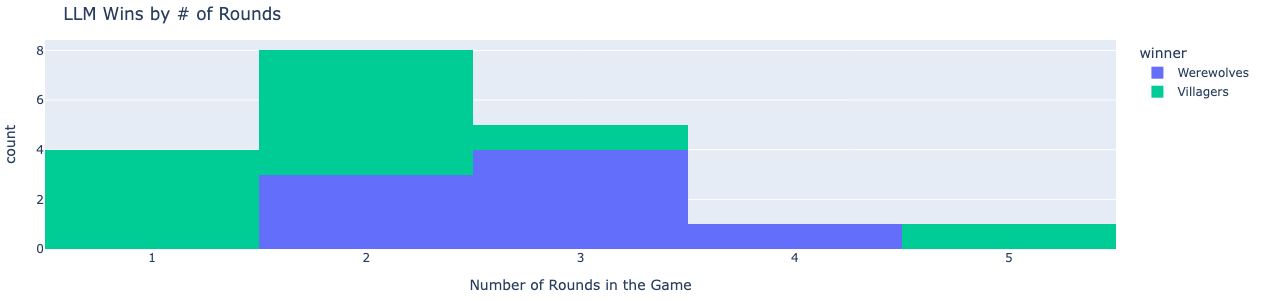
\includegraphics[keepaspectratio]{paper_files/figure-latex/Data-EDA_Comparison-fig-llm-winrounds-output-1.png}}

}

\caption{\label{fig-llm-winrounds}The LLM wins, by how many rounds that
partiticular game had.}

\end{figure}%

\end{minipage}%

\end{figure*}%

\section{Persuasion Strategies}\label{persuasion-strategies}

\begin{figure*}

In Figure~\ref{fig-strat-overall}, we compare the distribution of
persuasion strategies employed by humans and LLM agents across all
utterances. Human players display a diverse mix of techniques, with many
utterances containing no overt strategy and the rest spread across
interrogation, accusation, defense, and identity claims. In stark
contrast, LLM agents overwhelmingly default to a Call to Action strategy
--- direct exhortations or voting prompts --- with minimal use of
defensive language.

\begin{figure}[H]

\centering{

\pandocbounded{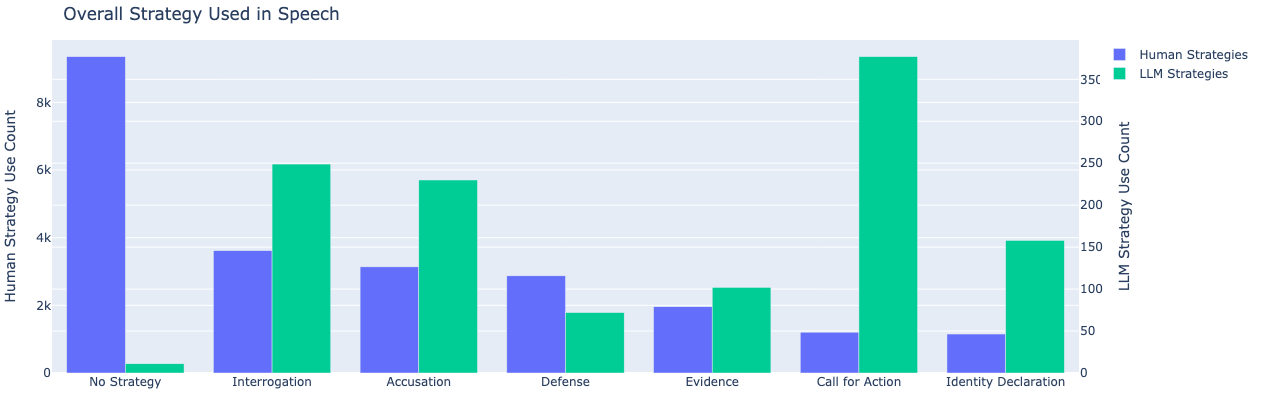
\includegraphics[keepaspectratio]{paper_files/figure-latex/Data-EDA_Comparison-fig-strat-overall-output-1.png}}

}

\caption{\label{fig-strat-overall}The persuasion strategies used by
humans vs LLMs; scales are seperate per dataset for more even
comparison.}

\end{figure}%

\end{figure*}%

Figure~\ref{fig-stratbyrole-hum} and Figure~\ref{fig-stratbyrole-llms}
reveal how strategy preferences vary by player role, scaled by each
role's strategy use (for more understandable analysis). Human Villagers,
Werewolves, Seers, and Doctors all rely heavily on Interrogation,
followed by Accusation and then Defense; notably, Villagers stand out
with a higher incidence of Identity Declaration, likely reflecting their
need to build trust through role claims. Among LLM agents, Call to
Action dominates every role, though Werewolves use Interrogation more
frequently than their counterparts and Doctors uniquely favor Defense
over Evidence when justifying their night actions.

\begin{figure*}

\begin{minipage}{0.50\linewidth}

\begin{figure}[H]

\centering{

\pandocbounded{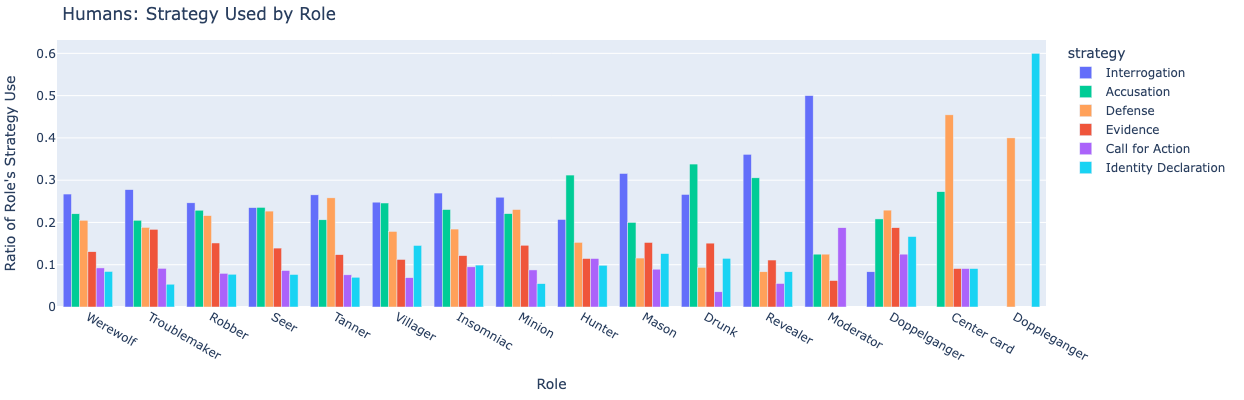
\includegraphics[keepaspectratio]{paper_files/figure-latex/Data-EDA_Comparison-fig-stratbyrole-hum-output-1.png}}

}

\caption{\label{fig-stratbyrole-hum}}

\end{figure}%

\end{minipage}%
%
\begin{minipage}{0.50\linewidth}

\begin{figure}[H]

\centering{

\pandocbounded{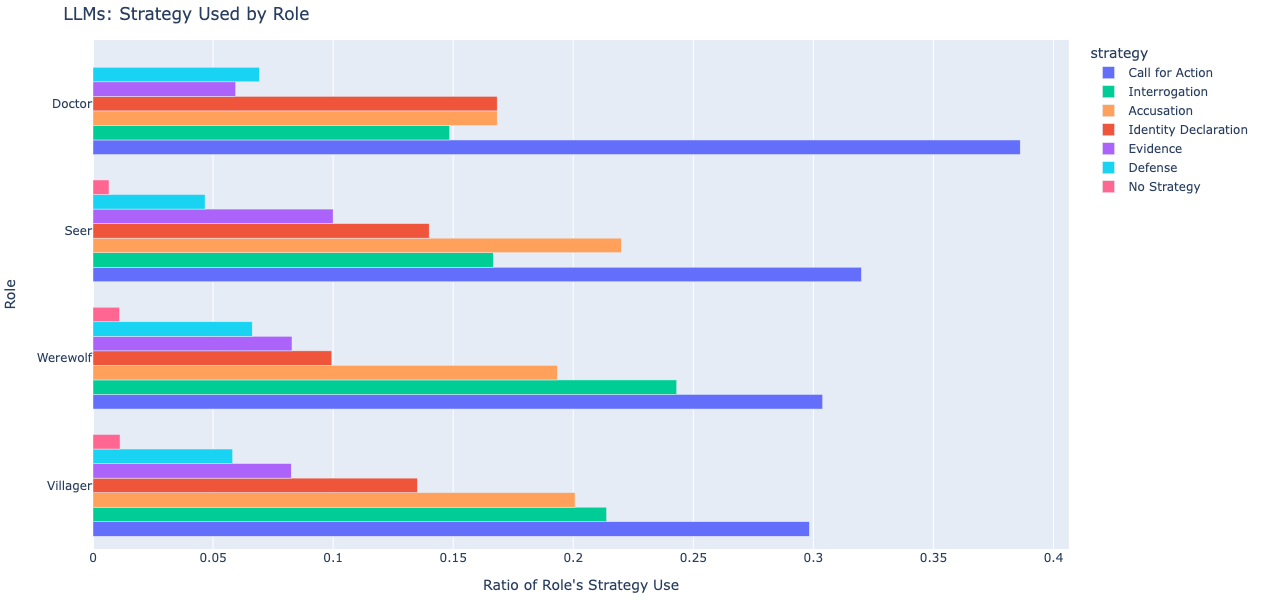
\includegraphics[keepaspectratio]{paper_files/figure-latex/Data-EDA_Comparison-fig-stratbyrole-llms-output-1.png}}

}

\caption{\label{fig-stratbyrole-llms}}

\end{figure}%

\end{minipage}%

\end{figure*}%

\begin{figure*}

\begin{figure}[H]

\centering{

\pandocbounded{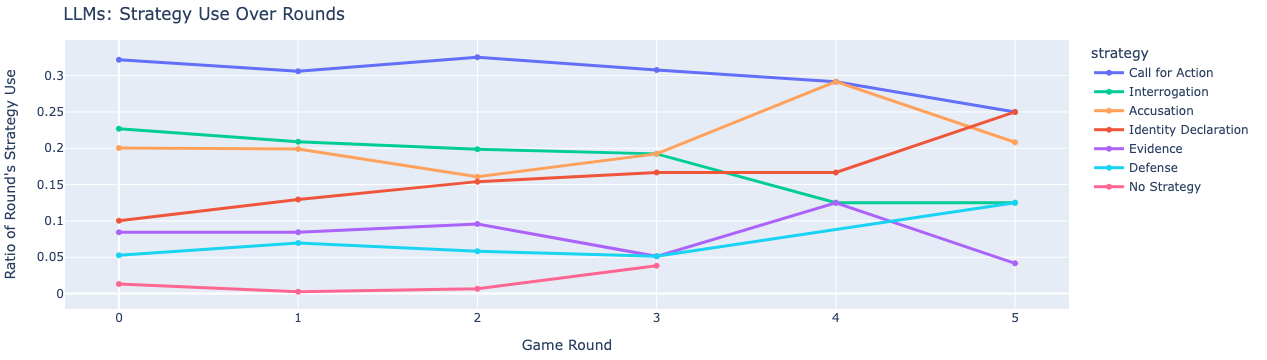
\includegraphics[keepaspectratio]{paper_files/figure-latex/Data-EDA_Comparison-fig-llm-stratbyround-output-1.png}}

}

\caption{\label{fig-llm-stratbyround}}

\end{figure}%

Figure~\ref{fig-llm-stratbyround} examines how LLM persuasion evolves
over the course of a game. Early rounds are marked by intense Call to
Action and Interrogation strategies, as agents strive to influence
voting and gather information. As discussions progress, these approaches
wane, giving way to increased Identity Declarations, Accusations, and
Defenses, indicating a shift toward justification and reputation
management in later rounds.

\end{figure*}%

\section{Voting Patterns}\label{voting-patterns}

To assess whether speaking volume influences suspicion, we plotted vote
frequency against utterance count in Figure~\ref{fig-talking-hum} and
Figure~\ref{fig-talking-llm}. Human players who speak more often are
indeed more likely to be targeted in votes, suggesting a bias against
the most vocal participants. LLM agents, however, show little to no
correlation between talkativeness and vote count, indicating more
uniform voting behavior irrespective of individual participation levels.

\begin{figure*}[H]

\centering{

\pandocbounded{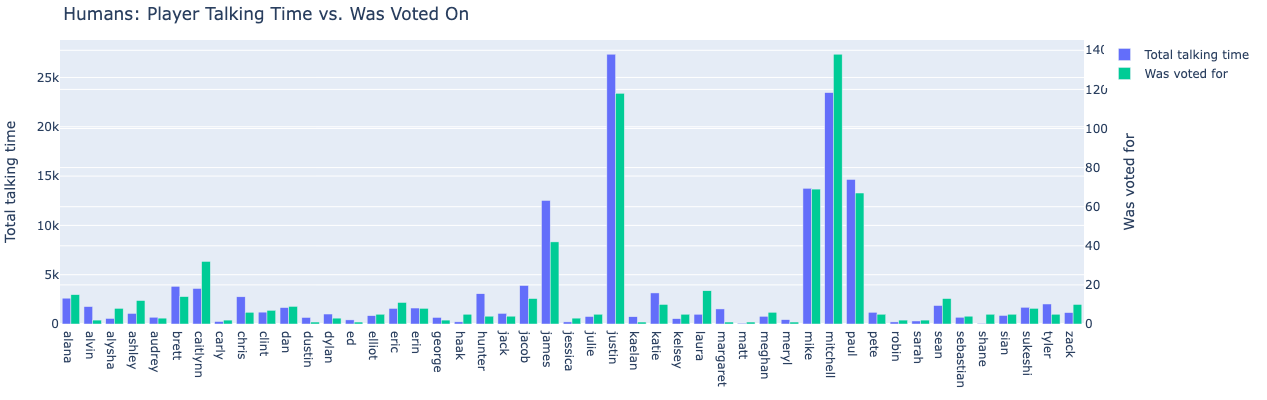
\includegraphics[keepaspectratio]{paper_files/figure-latex/Data-EDA_Comparison-fig-talking-hum-output-1.png}}

}

\caption{\label{fig-talking-hum}}

\end{figure*}%

\begin{figure*}[H]

\centering{

\pandocbounded{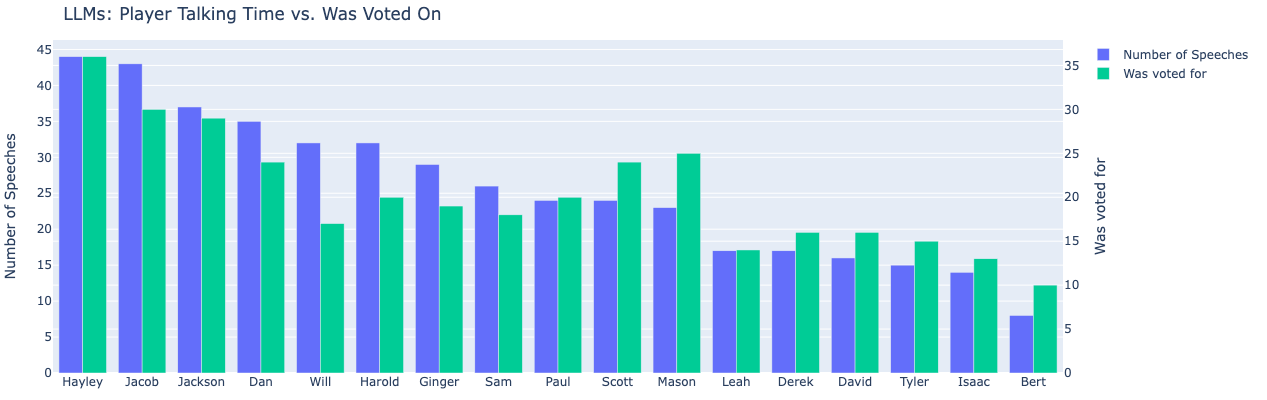
\includegraphics[keepaspectratio]{paper_files/figure-latex/Data-EDA_Comparison-fig-talking-llm-output-1.png}}

}

\caption{\label{fig-talking-llm}}

\end{figure*}%

\begin{figure*}

Figure~\ref{fig-voting-spread} presents the distribution of vote
concentration per round, measured as the ratio of players voting for the
most popular choice. Human voting patterns are highly variable: some
rounds feature unanimous consensus, while others show completely
scattered votes. In contrast, LLM agents demonstrate more consistency,
with 25\%--85\% of votes typically aligning on the top candidate each
round, reflecting predictable decision rules embedded in their prompts
and bidding mechanism.

\begin{figure}[H]

\centering{

\pandocbounded{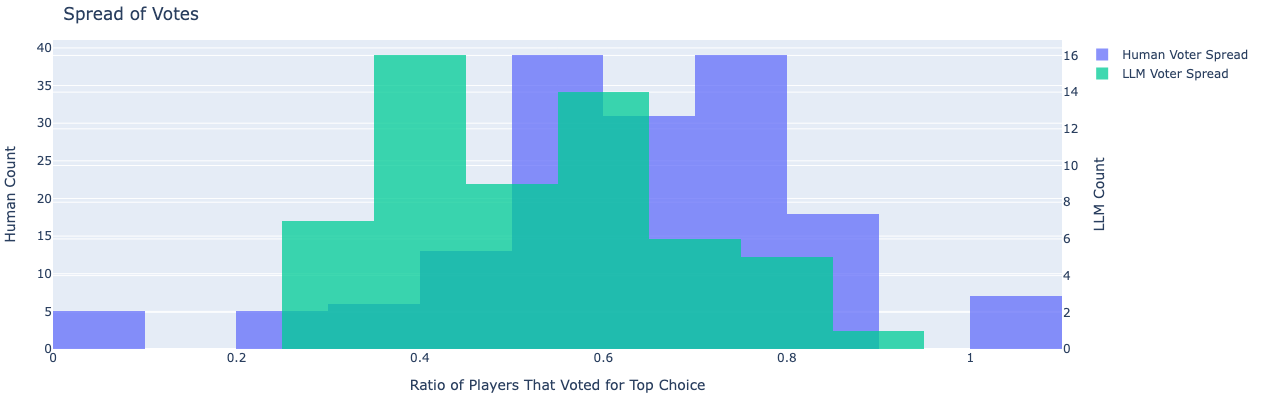
\includegraphics[keepaspectratio]{paper_files/figure-latex/Data-EDA_Comparison-fig-voting-spread-output-1.png}}

}

\caption{\label{fig-voting-spread}}

\end{figure}%

\end{figure*}%

\chapter{Discussion and Conclusion}\label{discussion-and-conclusion}

Our comparative analysis reveals that LLM-driven agents not only
outperform human players in terms of villager win rates but also exhibit
markedly different strategic and behavioral patterns. The higher success
rate of LLM villagers---winning nearly 58\% of games versus 37\% for
humans---suggests that LLMs are particularly adept at early-round
coordination and deduction. This is reinforced by the round-by-round win
dynamics: LLM villagers overwhelmingly secure victories within the first
two discussion rounds, indicating a strong capacity for rapid consensus
building. In contrast, human teams often extend the game, perhaps
reflecting a mix of uncertainty and exploratory dialogue that delays
definitive accusations. These findings imply that while humans may
engage in richer, more varied conversation, LLMs leverage their
prompt-driven ``Call to Action'' strategy to focus discussions quickly
around voting decisions, thereby minimizing the window for deception.

However, the dominance of a single persuasion strategy among LLMs also
highlights important limitations. Unlike humans---who deploy a balanced
repertoire of interrogation, accusation, defense, and identity
declarations---LLM agents overwhelmingly resort to direct exhortations
or voting prompts, with minimal defensive or evidentiary reasoning. This
narrow strategic palette may contribute to their early-round success yet
also points to a lack of adaptive nuance; for instance, LLM werewolves
struggle to sustain deception over multiple rounds and rely less on
subtle tactics such as identity claims or evidence-based persuasion.
Similarly, the voting behavior of LLMs, which shows a consistent
25--85\% alignment on the top choice each round, contrasts with the
broad variability observed in human votes and suggests that agent
prompting enforces uniformity at the expense of authentic deliberation.
Taken together, these insights underscore both the strengths and the
rigidities of current LLM architectures in social deduction contexts:
they excel at swift coordination under structured prompts, but they lack
the flexible, context-sensitive judgment that characterizes human
strategic interplay. Future work should explore hybrid approaches that
blend the decisiveness of LLM-driven voting with the expressive
diversity of human persuasion strategies to achieve both efficiency and
depth in adversarial group interactions.

\section{Limitations}\label{limitations}

Despite the insights gained, our study has several important
limitations. First, the number of LLM-simulated games was constrained by
per-call API costs, resulting in only 19 simulated matches versus 163
human games. This small sample increases variance in the LLM win‐rate
estimates and may obscure subtler patterns of strategic behavior.
Second, our manual annotation of LLM utterances for persuasion
strategy---while guided by the same taxonomy as the human dataset---was
necessarily more cursory than the fully expert-validated labels in the
Werewolf Among Us corpus. As a result, some nuanced tactics or
mixed‐strategy turns may have been misclassified or overlooked.

Additionally, the human dataset itself differs from our LLM simulations
in fundamental ways: it consists of one-round ``One Night'' variants
with specialized roles and no eliminations, whereas the LLM Arena
follows classic multi-round Werewolf rules with eliminations and night
actions. These structural differences complicate direct comparisons of
strategy prevalence and win dynamics. Finally, all LLM agents relied on
a fixed prompt design and bidding mechanism that may bias them toward
certain behaviors (e.g., frequent calls to action); alternative prompt
formulations or interactive interfaces could yield different outcomes.

\section{Future Work}\label{future-work}

To address these limitations, future research should expand the scale
and diversity of LLM simulations by negotiating lower API costs or
leveraging open-source models. A larger, more varied set of games would
enable finer-grained analysis of how model size, architecture, and cost
constraints interact with strategic performance. Concurrently, a more
rigorous annotation pipeline---potentially incorporating multi-rater
agreement or semi-automated classification---could improve the fidelity
of strategy labels for LLM dialogue.

We also recommend designing hybrid human--AI experiments in which human
players interact directly with LLM agents under controlled conditions.
Such studies would reveal how LLM persuasion strategies influence, and
are influenced by, real human responses. Exploring alternative prompt
structures, dynamic bidding rules, or reward signals (e.g.,
reinforcement learning to optimize for deceptive success) could further
uncover the boundaries of LLM social reasoning. Finally, extending this
comparative framework to other social deduction games or negotiation
tasks would test the generality of our findings across domains of trust,
cooperation, and adversarial persuasion.

\section{Summary}\label{summary}

In this work, we presented the first direct comparison of human and LLM
behavior in the classic Werewolf social deduction game. By aligning two
annotated datasets---Werewolf Among Us for humans and the
custom-simulated Werewolf Arena for LLMs---we evaluated win rates,
persuasion strategies, and voting dynamics across roles and rounds. Our
results demonstrate that LLM agents achieve higher villager win rates,
driven by early, prompt-focused ``Call to Action'' strategies, yet they
lack the adaptive nuance and strategic diversity characteristic of human
players.

These findings highlight both the promise and rigidity of current large
language models in group-level adversarial settings: they excel at rapid
coordination but underutilize defensive and evidence-based tactics. By
identifying key areas for improvement---such as more balanced strategy
repertoires, refined annotation methods, and human--AI hybrid
studies---we chart a roadmap for enhancing LLM social intelligence and
developing richer, more human-like agents in future research.

\begin{center}\rule{0.5\linewidth}{0.5pt}\end{center}

\chapter{References}\label{references}

\phantomsection\label{refs}
\begin{CSLReferences}{1}{0}
\bibitem[\citeproctext]{ref-bailisWerewolfArenaCase2024}
Bailis, Suma, Jane Friedhoff, and Feiyang Chen. 2024. {``Werewolf
{Arena}: {A Case Study} in {LLM Evaluation} via {Social Deduction}.''}
July 18, 2024. \url{https://doi.org/10.48550/arXiv.2407.13943}.

\bibitem[\citeproctext]{ref-chiAMONGAGENTSEvaluatingLarge2024}
Chi, Yizhou, Lingjun Mao, and Zineng Tang. 2024. {``{AMONGAGENTS}:
{Evaluating Large Language Models} in the {Interactive Text-Based Social
Deduction Game}.''} July 24, 2024.
\url{https://doi.org/10.48550/arXiv.2407.16521}.

\bibitem[\citeproctext]{ref-choRoundTableInvestigatingGroup2024}
Cho, Young-Min, Raphael Shu, Nilaksh Das, Tamer Alkhouli, Yi-An Lai,
Jason Cai, Monica Sunkara, and Yi Zhang. 2024. {``{RoundTable}:
{Investigating Group Decision-Making Mechanism} in {Multi-Agent
Collaboration}.''} November 11, 2024.
\url{https://doi.org/10.48550/arXiv.2411.07161}.

\bibitem[\citeproctext]{ref-duLargeLanguageModels2024}
Du, Yinuo, Prashanth Rajivan, and Cleotilde Gonzalez. 2024. {``Large
{Language Models} for {Collective Problem-Solving}: {Insights} into
{Group Consensus Decision-Making}.''} \emph{Proceedings of the Annual
Meeting of the Cognitive Science Society} 46 (0).
\url{https://escholarship.org/uc/item/6s060914}.

\bibitem[\citeproctext]{ref-laiWerewolfUsMultimodal2022}
Lai, Bolin, Hongxin Zhang, Miao Liu, Aryan Pariani, Fiona Ryan, Wenqi
Jia, Shirley Anugrah Hayati, James M. Rehg, and Diyi Yang. 2022.
{``Werewolf {Among Us}: {A Multimodal Dataset} for {Modeling Persuasion
Behaviors} in {Social Deduction Games}.''} December 16, 2022.
\url{https://doi.org/10.48550/arXiv.2212.08279}.

\bibitem[\citeproctext]{ref-piattiCooperateCollapseEmergence2024}
Piatti, Giorgio, Zhijing Jin, Max Kleiman-Weiner, Bernhard Schölkopf,
Mrinmaya Sachan, and Rada Mihalcea. 2024. {``Cooperate or {Collapse}:
{Emergence} of {Sustainable Cooperation} in a {Society} of {LLM
Agents}.''} \emph{Advances in Neural Information Processing Systems} 37
(December): 111715--59.
\url{https://proceedings.neurips.cc/paper_files/paper/2024/hash/ca9567d8ef6b2ea2da0d7eed57b933ee-Abstract-Conference.html}.

\bibitem[\citeproctext]{ref-stepputtis2023longhorizon}
Stepputtis, Simon, Joseph Campbell, Yaqi Xie, Zhengyang Qi, Wenxin
Sharon Zhang, Ruiyi Wang, Sanketh Rangreji, Charles Michael Lewis, and
Katia P. Sycara. 2023. {``Long-Horizon Dialogue Understanding for Role
Identification in the Game of Avalon with Large Language Models.''} In
\emph{Proceedings of the 2023 Conference on Empirical Methods in Natural
Language Processing}. \url{https://openreview.net/forum?id=JKmsjKJ0Q8}.

\bibitem[\citeproctext]{ref-wikiwerewolf}
Wikipedia contributors. 2024. {``Mafia (Party Game).''}
\url{https://en.wikipedia.org/wiki/Mafia_(party_game)}.

\bibitem[\citeproctext]{ref-xuLanguageAgentsReinforcement2024}
Xu, Zelai, Chao Yu, Fei Fang, Yu Wang, and Yi Wu. 2024. {``Language
{Agents} with {Reinforcement Learning} for {Strategic Play} in the
{Werewolf Game}.''} February 20, 2024.
\url{https://doi.org/10.48550/arXiv.2310.18940}.

\end{CSLReferences}

\begin{center}\rule{0.5\linewidth}{0.5pt}\end{center}

\chapter{Project Contributions}\label{project-contributions}

\textbf{Bhavana Jonnalagadda}:

\begin{itemize}
\tightlist
\item
  Paper framework (Quarto) setup
\item
  Github repo management
\item
  EDA on LLM dataset
\item
  Final comparison EDA and results analysis
\item
  Results section
\item
  Discussion and Conclusion section
\item
  Abstract
\end{itemize}

\textbf{Riley Jones}:

\begin{itemize}
\tightlist
\item
  EDA on human dataset
\item
  Werewolf Arena LLM simulation running and data aquisition
\item
  Introduction section
\item
  Methods section
\end{itemize}




\end{document}
